%aum ganathipathaye namaha
%sri rama jeyam
\section{Introduction}\label{sec:info}

%\ly{we should write it more general first for SE communities.}

Recently, binary code searching has attracted a lot of attentions for its important applications in software engineering and security,
%An effective binary searching tool can greatly help in various tasks to maintain the vitality of the software industry,
e.g.,  software plagiarism detection~\cite{luo2014semantics}, reverse engineering~\cite{caballero2009binary}, semantic recovery~\cite{kim2014reuse}, malware detection~\cite{ming2015memoized} and buggy (vulnerable) code identification~\cite{DBLP:conf/sp/PewnyGGRH15,DBLP:conf/pldi/DavidY14} in various software components where the source code is not available (e.g., legacy applications).
We can even search for zero-day vulnerabilities in proprietary binary by matching the known vulnerability from open source software.
%, in various software components for which the source code is not available (e.g., legacy application), have rise the demanded for scalable binary code searching techniques.
%recommend similar code solutions, identify binary semantics, and also reveal zero-day vulnerabilities. %Especially in software testing and security domain, vulnerabilities in software are deep hidden in inscrutable binary code, leaving a legacy ticking-time bomb in a software system.
%Especially, among the various vulnerability detection techniques~\cite{DBLP:journals/csur/ShahriarZ12}, binary code search is a fast yet accurate solution that preludes a further manual check of security experts.

Traditional source code search relies on the similarity analysis of some representations of source code, e.g., approaches based on token~\cite{DBLP:journals/tse/KamiyaKI02}, abstract syntax tree (AST) \cite{DBLP:conf/icse/JiangMSG07} or program dependency graph (PDG)~\cite{DBLP:conf/icse/GabelJS08}. All these representations capture the structural information of the program, and yield accurate results for source code search. However, code search in binary is much more challenging due to many factors (e.g., architecture and OS choice, compiler type, optimization level or even obfuscation technique) and limited availability of high-level program information. These factors have a substantial influence on the assembly instructions and their final layout in the compiled binary executable.

Recently, various approaches have been proposed to detect the similar binary code by using static or dynamic analysis.
%To better understand the mainstream binary function matching techniques,
Static analysis~\cite{DBLP:conf/pldi/DavidY14,saebjornsen2009detecting,luo2014semantics,DBLP:conf/sp/PewnyGGRH15} relies on the syntactical and structural information of binaries, especially control-flow structures (i.e., organization of basic blocks within a function) to perform the matching. % , and does not capture the true semantics (i.e., complete understanding) of the program under investigation.
Dynamic approaches~\cite{DBLP:conf/issta/JiangS09,DBLP:conf/asplos/Schkufza0A13,DBLP:conf/icse/JhiWJZLW11,DBLP:conf/uss/EgeleWCB14,egele2014blanket} inspect the invariants of input-output or intermediate values of program at runtime to check the equivalence of binary programs.
Table~\ref{tab:lit_rev} summarizes the state-of-the-art binary code search techniques proposed in the literature. \textsc{\small Tracy}~\cite{DBLP:conf/pldi/DavidY14} is a pure syntax based function matching technique
%(hence, true function seamntics are not captured)
that uses $n$-tracelet (i.e., basic blocks of length $n$ along the control-flow path), which is architecture- and OS-dependent. \textsc{\small CoP}~\cite{luo2014semantics} is a plagiarism detection tool that leverages on the theorem prover to search for semantically equivalent code segments.
%, hence, not very scalable for real-world binaries \mahin{and does not support cross-architecture and cross-OS analysis}.
The bug search tool proposed in~\cite{DBLP:conf/sp/PewnyGGRH15} supports cross-architecture analysis via the invariants of bug signatures.
%Since different OSs use different ABI (Application Binary Interface), \cite{DBLP:conf/sp/PewnyGGRH15} has very limited support for cross-OS analysis because of ignoring ABI in the analysis.
%Since extracting semantic features is quite expensive and there is no pre-filtering process in place to narrow down the search space,  \cite{DBLP:conf/sp/PewnyGGRH15} is not very scalable and in addition, due to incomplete modeling, it captures only the partial semantics of the functions.
%ABI in the analysis.
%Further, \textsc{\small CoP} and~\cite{DBLP:conf/sp/PewnyGGRH15} are program structure dependent, where they use pairwise basic-block similarity search as an initial step to identify candidate target functions that are similar to the signature\footnote{\mahin{define signature and target functions}}. This indicates that both \textsc{\small CoP} and~\cite{DBLP:conf/sp/PewnyGGRH15} have an implicit assumption that at least one basic-block is preserved in the signature and target binaries. These assumptions are too restrictive for real-world binaries especially, when the signature and target binaries (or fucntions) do not share the \mahin{same code base}.
\textsc{\small discovRE} tool~\cite{sebastian2016discovre} is proposed to find bugs in binaries across-architectures in a scalable manner, where it uses two filters (numeric and structural) to quickly locate the functions that appear similar \xyx{with} the signature function.
Finally, \textsc{\small BLEX}~\cite{egele2014blanket} is the latest dynamic function matching tool using seven semantic features.%, which captures the precise semantics of the binary code.
%As a dynamic analysis tool, \textsc{\small BLEX} %does code search at the function level
%is not scalable and, due to implementation limitations, does not support cross-architecture and cross-OS analysis.



%\begin{table*}[t]
%\scriptsize
%	\begin{center}
%\caption{Comparison of existing techniques} \label{tab:lit_rev}
%\begin{tabular}{ | m{2.1cm} |  m{1.2cm} | m{4cm} | m{2cm} | m{1.3cm} | m{2.5cm} |  m{1.0cm}| }
%\hline
%	\textbf{Tool} & \textbf{Technique} & \textbf{Similarity matching} & \textbf{Cross-architecture} & \textbf{Cross-OS} & \textbf{Complete  semantics} &  \textbf{Scalable} \\ \hline
%	 BLEX~\cite{egele2014blanket} & Dynamic & Whole-function matching &  Limited & Limited & Yes & No \\ \hline
%	 Tracy~\cite{DBLP:conf/pldi/DavidY14} & Static & Partial trace (fixed length) matching & No & No & No & Yes \\ \hline
%     CoP~\cite{luo2014semantics} & Static & Pairwise basic-block matching& No & No & No & No \\ \hline
%	Bug search~\cite{DBLP:conf/sp/PewnyGGRH15} & Static & Pairwise basic-block matching & Limited & Limited & No & Yes \\ \hline
%	discovRE~\cite{sebastian2016discovre} & Static & Pairwise basic-block matching & Limited & Limited & No & Yes \\ \hline
%	 BinGo & Static & Partial trace (variable length) matching & Yes & Yes & Yes &  Yes \\ \hline
%\end{tabular}
%\end{center} \vspace{-7mm}
%\end{table*}

%
%\begin{figure*}
%\CenterFloatBoxes
%\begin{floatrow}
%\ttabbox
%  {
%  \scriptsize
%  \begin{tabular}{ | m{1.6cm} | m{1.9cm} | m{1.9cm} | m{0.7cm} | }
%\hline
%	\textbf{Tool}  & \textbf{Rely on structural properties (C1)} & \textbf{Capture complete semantics (C2)} & \textbf{Scalable (C3)} \\ \hline
%	 BLEX~\cite{egele2014blanket} & No &  Yes & No \\ \hline
%	 Tracy~\cite{DBLP:conf/pldi/DavidY14}  & Yes & No & Yes \\ \hline
%     CoP~\cite{luo2014semantics} & Yes (initial step) & Limited (along the execution path only) & No  \\ \hline
%	Bug search~\cite{DBLP:conf/sp/PewnyGGRH15} & Yes & No & No  \\ \hline
%	discovRE~\cite{sebastian2016discovre}& Yes & No & Yes  \\ \hline
%	 BinGo & No & Yes & Yes \\ \hline
%  \end{tabular}
%  }
%  {\caption{Comparison of existing techniques} \label{tab:lit_rev}}
%  
%\ffigbox
%  {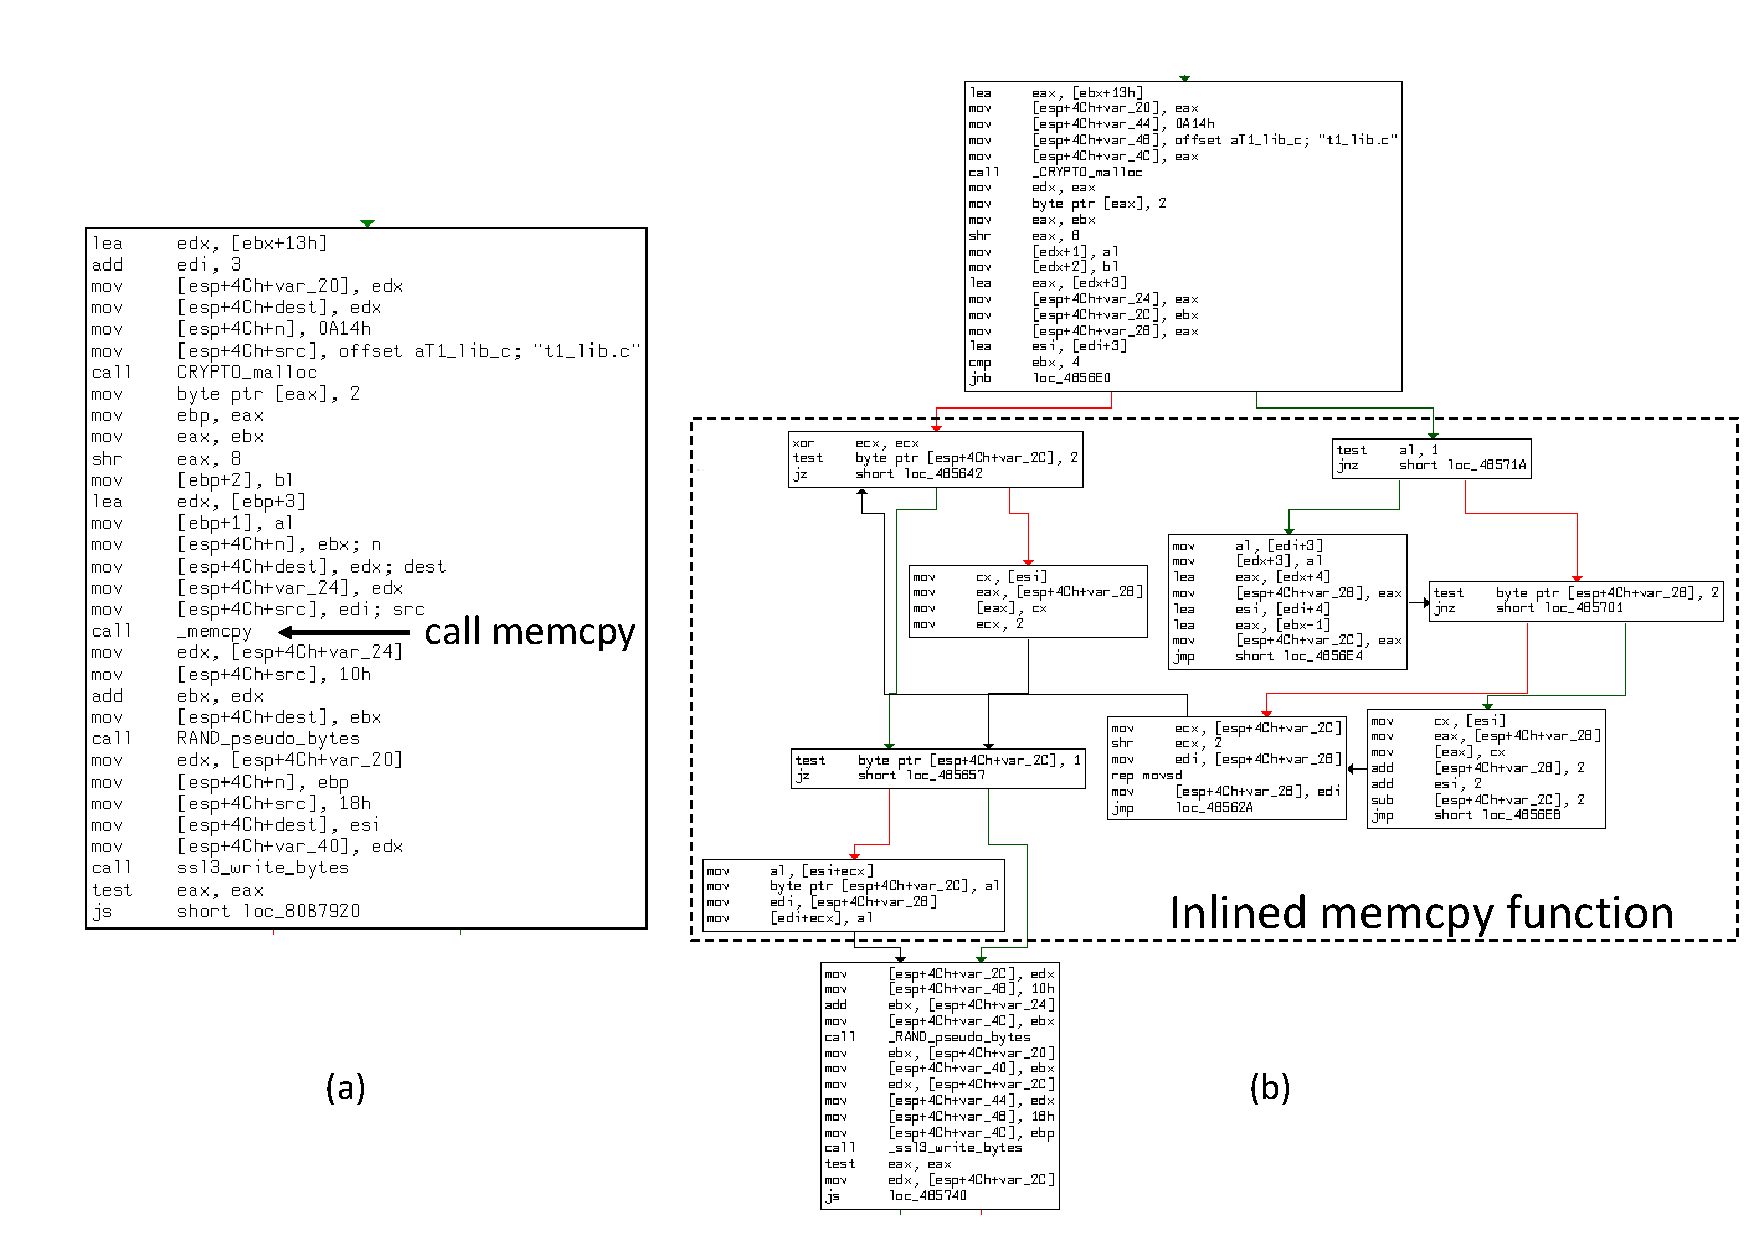
\includegraphics[width=\linewidth]{srj-figures/srj-moti_ex2.pdf}}
%  {\caption{Code segment responsible for Heartbleed vulnerability (CVE-2014-0160) appeared as in the binary (a) compiled with GCC 4.6, and (b) compiled with Mingw32} \label{fig:prob_stat}}
%\killfloatstyle
%
%\end{floatrow}
%\end{figure*}


\begin{table}[t]
\scriptsize
	\begin{center}
\caption{Comparison of existing techniques} \label{tab:lit_rev}
\begin{tabular}{ | m{1.6cm} | m{1.9cm} | m{1.9cm} | m{0.7cm} | }
\hline
	\textbf{Tool}  & \textbf{Rely on structural properties (C1)} & \textbf{Capture complete semantics (C2)} & \textbf{Scalable (C3)} \\ \hline
	 BLEX~\cite{egele2014blanket} & No &  Yes & No \\ \hline
	 Tracy~\cite{DBLP:conf/pldi/DavidY14}  & Yes & No & Yes \\ \hline
     CoP~\cite{luo2014semantics} & Yes (initial step) & Limited (along the execution path only) & No  \\ \hline
	Bug search~\cite{DBLP:conf/sp/PewnyGGRH15} & Yes & No & No  \\ \hline
	discovRE~\cite{sebastian2016discovre}& Yes & No & Yes  \\ \hline
	 BinGo & No & Yes & Yes \\ \hline
  \end{tabular}
  \end{center} \vspace{-7mm}
\end{table}


% followed by LCSSEBB\footnote{Longest common subsequence of semantically equivalent basic-block}
%followed by BHB\footnote{Best-Hit-Boarding algorithm

%Here, true semantics of a program (or function) refers to the complete understanding of the functionality of the program.
%\textsc{\small BLEX}~\cite{DBLP:conf/uss/EgeleWCB14} is the latest tool in this line, as it uses seven semantic features from an execution (e.g., calling imported library functions). %However, \textsc{\small BLEX} is for x64 binaries, not for cross-architecture code search. Pewny \emph{et al.} \cite{DBLP:conf/sp/PewnyGGRH15} propose a purely static analysis that can detect the similar code among  the binaries of the application on different OSs. This is good for finding clones of the same program due to architecture or compilation differences, but maybe not good at finding relaxed binary clones among different applications.

%These approaches can be effective, but they face challenges from two aspects: the difficulty in setting up the execution environment to dynamically execute, and the scalability issue that prevents large-scale analysis.
%In the following, we highlight the key limitations in the existing binary function matching techniques.
%Table~\ref{tab:lit_rev} shows that static approaches cannot precisely capture the full semantics, while dynamic methods struggle for the scalability.
%To have a better comparison, we list the key challenges that restrict the existing approaches.

%\mahin{In all the techniques listed in Table~\ref{tab:lit_rev}, it is implicitly assumed that both the signature and target binaries share (or forked from) the same code base. However, this assumption is too restrictive and have limited real-world applications \footnote{This assumption is justifiable for only \textsc{\small CoP} as it is a plagiarism detection technique}.}
%\mahin{In the techniques presented in Table~\ref{tab:lit_rev}, we find three key limitations and they are summarized below:}

%\renewcommand{\theenumi}{\arabic{enumi}}
Table~\ref{tab:lit_rev} shows that static approaches are not precise, while dynamic methods struggle for the scalability.
A deeper analysis shows that existing approaches face the following challenges.
\vspace{-2mm}
\begin{itemize}%[label=\textbf{P\arabic*.},itemindent=*,itemsep=0mm]
\itemsep0em
\item \textbf{C1.} The structural information used by the static approaches, e.g., basic-block structures used in~\cite{luo2014semantics,DBLP:conf/sp/PewnyGGRH15,sebastian2016discovre} and fixed length tracelet in \cite{DBLP:conf/pldi/DavidY14}, \xyx{is} not resilient to
%syntax gaps
\mahin{the structural differences} introduced due to architecture, OS and compiler differences.
\item \textbf{C2.}  Covering the complete function semantics is challenging for all static analysis techniques, which ignore the semantics of system libraries and user-defined functions in the matching.
\item \textbf{C3.} Considering the huge amount of target functions in the real world binaries, scalability is a great challenge in semantic binary search~\cite{luo2014semantics,DBLP:conf/sp/PewnyGGRH15}.
\end{itemize}
\vspace{-2mm}
%\ly{I am not happy with the following paragraph, let's discuss tmr.}

As elaborated further in Section \ref{sec:back:challenge}, the above challenge are the keys factors to achieve an accurate yet scalable cross-architecture and cross-OS binary search tool. Clearly, none of the existing techniques in Table~\ref{tab:lit_rev} solved all the challenges above.

%\textbf{P1} requires the solution to be architecture- and OS- neutral, and be resistant to the variances that arise due to the differences in compiler type and optimization level.
%Static techniques based on the structural properties of binary functions will fail~\cite{DBLP:conf/pldi/DavidY14,luo2014semantics,DBLP:conf/sp/PewnyGGRH15,sebastian2016discovre}.
%Most of the static analysis also assume that the functions are self-contained (i.e., invocations of libraries and other user-defined functions are ignored). Thus the true function semantics are not fully captured~\cite{DBLP:conf/pldi/DavidY14,DBLP:conf/sp/PewnyGGRH15, sebastian2016discovre}.
%Lastly, scalability still requires more efforts to avoid matching every single target function in the database~\cite{egele2014blanket,DBLP:conf/pldi/DavidY14,luo2014semantics,DBLP:conf/sp/PewnyGGRH15}.

%This work aims at addressing the limitations to build a robust, scalable binary code searching (or function matching) tool that can support cross-architecture, OS and compiler (with various optimization levels) analysis with less (no) assumptions on the nature of signature and target binaries.  To this end, we design an approach to address the aforementioned problems with the following merits.

In this paper, we propose a binary function searching framework, named \tool, which combines a set of key techniques to address the challenges above. %: selective inlining to recover binary semantics (for \textbf{C2}), function models consisting of partial traces of variant lengths (for \textbf{C1}), and three filtering methods to scale the binary search (for \textbf{C3}).
Given a binary function, \tool first inlines relevant libraries and user-defined functions
%in the binary code
in order to capture the complete semantics of the function (for solving C2), then
shortlists the candidate target functions using an architecture and OS neutral filtering technique (for solving C3), and finally extracts the partial traces of various lengths from the candidate target functions as function models (for solving C1) and conducts the function similarity matching using machine learning technqiues.
%then extracts the partial traces of different lengths from the inlined binary as the function model (for solving C1), and finally filters infeasible traces and conducts the function match for similarity scoring (for solving C3).




%\noindent\textbf{Proposed solution.}

%\ly{need to describe the flow first and then to address the different challenges}

Technically, first, to recover the  complete semantics from the functions under investigation, we propose a \emph{selective inlining} technique, where the callee (both system libraries and user-defined) functions are inlined into the caller such that the complete function semantics are captured~\cite{wang2015binary} (See Section~\ref{sec:inline}). %without causing any code size explosion
To avoid code size explosion, we selectively inline the callee functions based on the invocation dependency patterns, which is very different from the traditional compiler inlining optimization techniques for maximum speed or minimum size~\cite{chang1992profile}.
To our best knowledge, this work is the first attempt towards the discussion of selective inlining in recovering binary semantics.
%\xyx{To mitigate the above problems, a solution is desired with the three following goals.} First, it should be architecture- and OS- neutral, and be resistant to the variances that arise due to the differences in compiler type and optimization level (for \textbf{P1}). \xyx{Second, it should be able to extract true semantics from the functions --- recover the complete functionality semantics  (for \textbf{P2}).} %identify semantically similar functions in binaries that stem from totally different code base, programming style and conventions (e.g., \texttt{libc} and \texttt{msvcrt}).}
%Finally, it should be scalable to real world binaries, avoiding to match every single target function in the database (for \textbf{P3}).
%

%%\xyx{Inlining is an effective solution for recovering the  function semantics [??]. However, deciding what functions need to be inlined is a critical problem --- a fundamental problem also faced by the compilers, where functions are selected to be inlined, during the compilation process, in order to optimize the binaries for maximum speed or minimum size~\cite{chang1992profile}. In general, binary code search and compilation have different goals for inlining decision.} %Compilers have access to high-level programming constructs from source code and their inlining decision is influenced by various factors such as user-defined \mahin{\texttt{INLINE} pragmas}, target function body-size, call-size (i.e., overhead required to invoke the function), saving estimation (i.e., estimated shrink in binary after inline), effects on caching, paging and register pressure~\cite{chang1992profile}. On the contrary, in binary code search,
%In binary analysis, to help recover binary semantics, inlining decision needs to made with the minimum possible information (no debugging information) available from the stripped binaries.

Second, to improve the scalability of our approach, we propose an \emph{architecture and OS neutral filtering} technique that narrows down the search space by shortlisting the candidate target functions for semantic similarity matching \xyx{(See Section~\ref{sec:prefilter})}.

Next, to overcome the limitation of basic-block structures (see Section 2.1), we generate \emph{function models}, which are agnostic to the underlying program structure, via the length variant partial traces\footnote{A partial trace refers to a sequence of basic-blocks that lie along an execution path in the CFG~\cite{DBLP:conf/pldi/DavidY14}.} (called, partial traces of \emph{k} lengths). For each function, \xyx{partial traces of length $1$ to $k$} are extracted to form the function model such that it represents the function at various granularity levels.
Here, we also take measure to minimize the effects of infeasible paths and compiler specific code in measuring the function similarity scores.

Finally, semantic features are extracted from the function models of candidate target functions, for function similarity scoring, where semantic features capture the machine state transitions in the form of Input/Output pairs (See Section~\ref{sec:func_match}).

%Next,  Finally, we also take measure to minimize the effects of infeasible paths and compiler specific code in measuring the function similarity scores.

\noindent\textbf{Experimental results.} We evaluate \tool on a number of real-world binaries with containing hundreds of thousands of functions.
The experimental results show that \tool can effectively perform cross-architecture and cross-OS binary code search on these binaries. \mahin{
\tool further comprehensively outperforms those the state-of-the-art tools, \textsc{\small Tracy}~\cite{DBLP:conf/pldi/DavidY14} and \textsc{\small BinDiff}~\cite{DBLP:conf/dimva/Flake04} for the same tasks. Further, we also show that recent techniques such as~\cite{DBLP:conf/sp/PewnyGGRH15} and~\cite{sebastian2016discovre}, fail when program structure is distorted, while \tool can handle such cases swiftly.}
%\xyx{??Mahin, we can mention how good our approach at matching binary that share no code base in a cross-architecture and cross-OS manner.}
Last but not least, using \tool, we \xyx{identify} a zero-day vulnerability (CVE-2016-0933) in the Adobe PDF Reader, an off-the-shelf commercial software.\\

\noindent\textbf{Key contributions.} In summary, we make the following contributions:
\begin{itemize}[nolistsep]
\itemsep0em
\item We propose a selective inlining algorithm to capture the complete semantic of the binary functions.
\item We introduce an architecture and OS neutral function filtering process that helps narrow down the target function search space.
\item We leverage on \emph{k}-length partial traces to model the function at various granularity levels that is agnostic to underlying program structures.
\item We empirically demonstrate that \tool outperforms the available state-of-the-art tools of binary code search, and report the identified zero-day vulnerabilities from COT binaries.%we also show that \tool can be used to hunt zero-day vulnerabilities from COT binaries.
\end{itemize}

